\section{Validation Results}
\label{sec:ValidationResults}

\subsection{Trade off Aperture and Power}
\label{sec:PowerApertureTradeoff}

In order to correctly determine the lasing power and the sizing of the receiver aperture, an optimization problem was created. This problem describes how the sizing of both the laser and receiver relate to the total amount of received photons. The method used to solve this problem is the Nelder-Mead (or downhill simplex) method as implemented is the Apache Commons Math library.

The most important parameter is the target amount of photons per pulse per satellite. This reflects the quality of the data. The target is set to 10 photons detected per transmitted pulse, as this will guaranty a decent quality in the BRDF reconstruction. As initial parameters, a power of 5W and an aperture of $10\times10$ cm are used. The performance of each iteration is quantified using the equation \ref{eq:PowerAperturePerformance}:

\begin{equation}
	\text{perf} = \frac {f(\varphi_{total}, \varphi_{target} \times \text{\# sats}, 50) \times 
												\displaystyle\prod_{sat} f(\varphi_{sat}, \varphi_{target}, 200) }
											{ \text{power} \times \text{aperture}^{1.2}}
	\label{eq:PowerAperturePerformance}
\end{equation}

In this equation, f(x, mean, variance) is a normal distribution given mean and variance evaluated at x. A visualization of the results can be seen in figure \ref{fig:PowerAperturePerformance}. It shows the region around the local maximum for the performance function. The results from the optimization algorithm in summary:

\begin{itemize}
	\item Power 4.6W
	\item Aperture 0.0045 m$^2$ (or $6.7\times6.7$ cm)
\end{itemize}

\begin{figure}[ht]
	\centering
	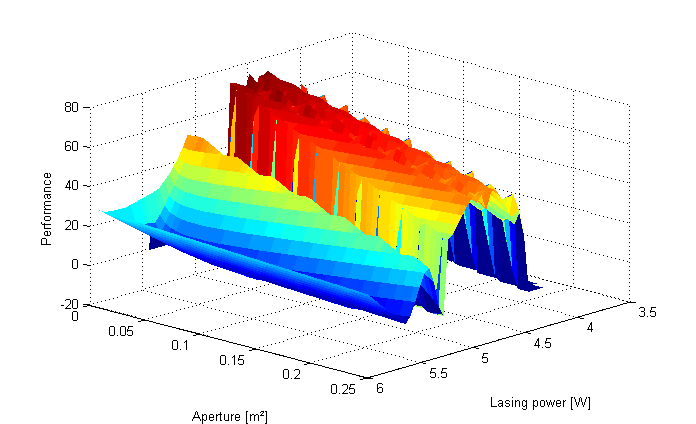
\includegraphics[width=0.6\textwidth]{optimize-PowerAperture.png}%
		\caption{Power-Aperture optimization visualization}%
		\label{fig:PowerAperturePerformance}%
\end{figure}

Note, these results are the bare minimum for the system to operate as designed. When taking a safe margin, this translates into a minimal lasing power of 5.5W and an aperture of 0.0055 m$^2$ ($7.5\times7.5$ cm). 

\subsection{Height Reconstruction}
\label{sec:HeightReconstruction}

Dropping a pingpong ball from LR and measure its travel time

\subsection{BRDF Reconstruction}
\label{sec:BRDFReconstuction}

One on three chance of rain


